\documentclass[aspectratio=169]{../latex_main/tntbeamer}  % you can pass all options of the beamer class, e.g., 'handout' or 'aspectratio=43'
\usepackage{dsfont}
\usepackage{bm}
\usepackage[english]{babel}
\usepackage[T1]{fontenc}
%\usepackage[utf8]{inputenc}
\usepackage{graphicx}
\graphicspath{ {./figures/} }
\usepackage{algorithm}
\usepackage[ruled,vlined,algo2e,linesnumbered]{algorithm2e}
\usepackage{hyperref}
\usepackage{booktabs}
\usepackage{mathtools}

\usepackage{amsmath,amssymb}

\DeclareMathOperator*{\argmax}{arg\,max}
\DeclareMathOperator*{\argmin}{arg\,min}

\usepackage{pgfplots}
\pgfplotsset{compat=1.16}
\usepackage{tikz}
\usetikzlibrary{trees} 
\usetikzlibrary{shapes.geometric}
\usetikzlibrary{positioning,shapes,shadows,arrows,calc,mindmap}
\usetikzlibrary{positioning,fadings,through}
\usetikzlibrary{decorations.pathreplacing}
\usetikzlibrary{intersections}
\pgfdeclarelayer{background}
\pgfdeclarelayer{foreground}
\pgfsetlayers{background,main,foreground}
\tikzstyle{activity}=[rectangle, draw=black, rounded corners, text centered, text width=8em]
\tikzstyle{data}=[rectangle, draw=black, text centered, text width=8em]
\tikzstyle{myarrow}=[->, thick, draw=black]

% Define the layers to draw the diagram
\pgfdeclarelayer{background}
\pgfdeclarelayer{foreground}
\pgfsetlayers{background,main,foreground}

% Requires XeLaTeX or LuaLaTeX
\usepackage{unicode-math}

\usepackage{fontspec}
%\setsansfont{Arial}
\setsansfont{RotisSansSerifStd}[ 
Path=../latex_main/fonts/,
Extension = .otf,
UprightFont = *-Regular,  % or *-Light
BoldFont = *-ExtraBold,  % or *-Bold
ItalicFont = *-Italic
]
\setmonofont{Cascadia Mono}[
Scale=0.8
]

% scale factor adapted; mathrm font added (Benjamin Spitschan @TNT, 2021-06-01)
%\setmathfont[Scale=1.05]{Libertinus Math}
%\setmathrm[Scale=1.05]{Libertinus Math}

% other available math fonts are (not exhaustive)
% Latin Modern Math
% XITS Math
% Libertinus Math
% Asana Math
% Fira Math
% TeX Gyre Pagella Math
% TeX Gyre Bonum Math
% TeX Gyre Schola Math
% TeX Gyre Termes Math

% Literature References
\newcommand{\lit}[2]{\href{#2}{\footnotesize\color{black!60}[#1]}}

%%% Beamer Customization
%----------------------------------------------------------------------
% (Don't) Show sections in frame header. Options: 'sections', 'sections light', empty
\setbeamertemplate{headline}{empty}

% Add header logo for normal frames
\setheaderimage{
	% 
\includegraphics[height=\logoheight]{figures/TNT_darkv4.pdf}
	
\includegraphics[height=\logoheight]{../latex_main/figures/luh_logo_rgb_0_80_155.pdf}
	% 
\includegraphics[height=\logoheight]{figures/logo_tntluh.pdf}
}

% Header logo for title page
\settitleheaderimage{
	% 
\includegraphics[height=\logoheight]{figures/TNT_darkv4.pdf}
	
\includegraphics[height=\logoheight]{../latex_main/figures/luh_logo_rgb_0_80_155.pdf}
	% 
\includegraphics[height=\logoheight]{figures/logo_tntluh.pdf}
}

% Title page: tntdefault 
\setbeamertemplate{title page}[tntdefault]  % or luhstyle
% Add optional title image here
%\addtitlepageimagedefault{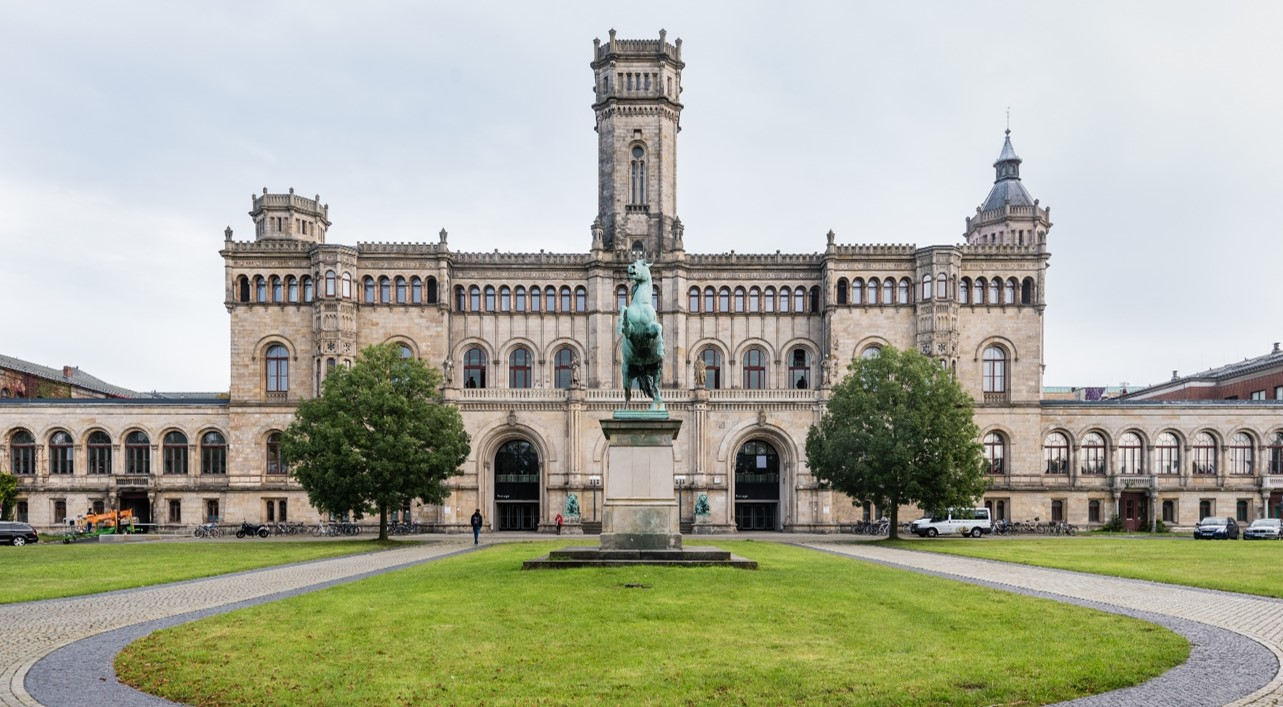
\includegraphics[width=0.65\textwidth]{figures/luh_default_presentation_title_image.jpg}}

% Title page: luhstyle
% \setbeamertemplate{title page}[luhstyle]
% % Add optional title image here
% \addtitlepageimage{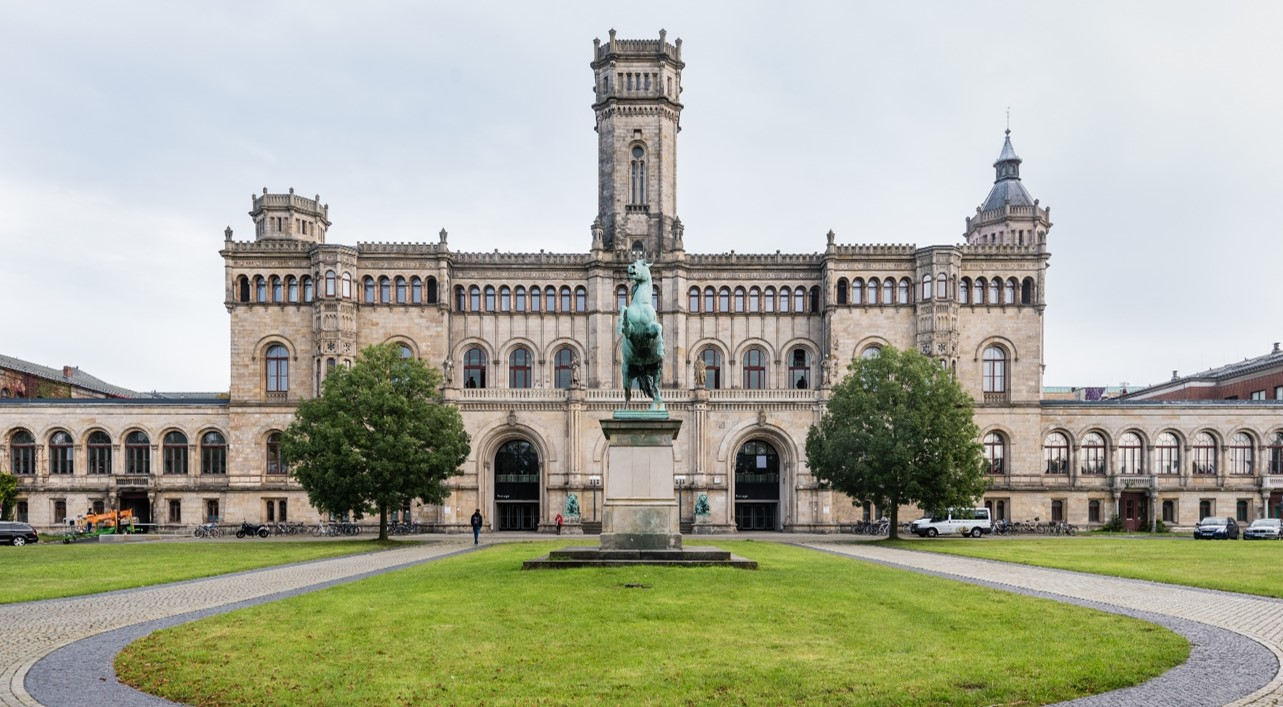
\includegraphics[width=0.75\textwidth]{figures/luh_default_presentation_title_image.jpg}}

\author[Lindauer \& Anand]{Marius Lindauer and Avishek Anand\\[1em]
	
\includegraphics[height=\logoheight]{../latex_main/figures/luh_logo_rgb_0_80_155.pdf}\qquad

\includegraphics[height=\logoheight]{../latex_main/figures/TNT_darkv4}\qquad

\includegraphics[height=\logoheight]{../latex_main/figures/L3S.jpg}	}
\date{Winter Term 2021
}


%%% Custom Packages
%----------------------------------------------------------------------
% Create dummy content
\usepackage{blindtext}

% Adds a frame with the current page layout. Just call \layout inside of a frame.
\usepackage{layout}


\title[Conclusion]{iML: Master Theses Pitches}
\subtitle{}

%\institute{}


\begin{document}
	
	\maketitle

	%-----------------------------------------------------------------------------------------------------------------------------


\begin{frame}[c]{Combining Hyperparameter Importance Methods}
 
	\begin{itemize}
		\item Level: BSc/MSc Thesis
		\item Idea in a nutshell:
		\begin{itemize}
		    \item On the meta-level, understanding the importance of hyperparamters to achieve peak performance is crucial
		    \item Different methods (e.g.. Ablation studies, fANOVA, ...) have different pros and cons 
		    \item Can we combine/ensemble these into a new technique showing the agreement and disagreement of different techniques? 
		\end{itemize}
		\item Requirements: Python, Hands-on ML, 
		\item Optional: AutoML
		\item Supervisor: Ren\'e Sass
	\end{itemize}
\end{frame}

\begin{frame}[c]{Robustness Assessment by Counterfactuals}
 
	\begin{itemize}
		\item Level: MSc Thesis
		\item Idea in a nutshell:
		\begin{itemize}
		    \item Robustness and better generalization is key for ML \& DL models
		    \item One way of increasing robustness is via setting the hyperparameter and architectural configuration
		    \item In this space, we can also apply counterfactuals (and also other iML approaches) to study how robust returned configurations are
		\end{itemize}
		\item Requirements: Python, Hands-on DL
		\item Optional: AutoML
		\item Supervisor: Ren\'e Sass
	\end{itemize}
\end{frame}

\begin{frame}[c]{Integration of Hyperparameter Importance in the Optimization Process}
 
	\begin{itemize}
		\item Level: MSc Thesis
		\item Idea in a nutshell:
		\begin{itemize}
		    \item For optimizing the hyperparameters of a ML model, we train an internal surrogate model (mapping hyperparameter configurations to loss)
		    \item Implicitly these surrogate models can learn how important hyperparameters are 
		    \item Can we make this knowledge more explicit and integrate it into the optimization process to early on focus on the important ones
		\end{itemize}
		\item Requirements: Python, Hands-on DL, AutoML
		\item Supervisor: Ren\'e Sass
	\end{itemize}
\end{frame}

\begin{frame}[c]{Meta-Models to Explain AutoML Surrogates}
 
	\begin{itemize}
		\item Level: MSc Thesis
		\item Idea in a nutshell:
		\begin{itemize}
		    \item For optimizing the hyperparameters of a ML model, we train an internal surrogate model (mapping hyperparameter configurations to loss)
		    \item Meta-Models can be used to make a (regression) model explainable by returning an explicit equation
		    \item Can we apply meta-models to make AutoML surrogate models interpretable?
		    \item We have to look out for the bias in our meta-data generation process
		\end{itemize}
		\item Requirements: Python, Hands-on DL, AutoML
		\item Supervisor: Ren\'e Sass
	\end{itemize}
\end{frame}

\begin{frame}[c]{Partial-Space Priors for Reusing Knowledge from AutoML Runs}
 
	\begin{itemize}
		\item Level: MSc Thesis
		\item Idea in a nutshell:
		\begin{itemize}
		    \item AutoML approaches can be deployed several times on similar datasets
		    \item This allows us to transfer knowledge as priors between AutoML runs to make future AutoML more efficient
		    \item However, can we still do this if the configuration space slightly changed (e.g., another hyperparameter was added)?
		    \item How can we design reasonable priors for Bayesian Optimization that takes into account unseen hyperparameters or task induced differences in the loss surface?
		\end{itemize}
		\item Requirements:
		\item Supervisor: Tim Ruhkopf
	\end{itemize}
\end{frame}

\begin{frame}[c]{Time Series Forecasting Ensemble: Auto-Correlation}
 
	\begin{itemize}
		\item Level: MSc Thesis
		\item Idea in a nutshell:
		\begin{itemize}
		    \item Time series forecasting is important in many applications\\ (e.g., weather, medicine, logistics, traffic, ...)
		    \item Some sequences mioght be auto-correlated (e.g., traffic flow at two neighboring traffic lights)
		    \item Exploit this characteristic of the data and train different DNN models (by using AutoML) and ensemble them 
		\end{itemize}
		\item Requirements: Python, DL hands-on
		\item Optional: AutoML
		\item Supervisor: Difan Deng
	\end{itemize}
\end{frame}

\begin{frame}[c]{Report Analysis Tool for AutoML}
 
	\begin{itemize}
		\item Level: BSc/MSc Thesis
		\item Idea in a nutshell:
		\begin{itemize}
		    \item AutoML tools often return only a single optimized hyperparameter configuration and neural architecture
		    \item To be able to trust the AutoML tools, users require more ways to interact with AutoML and more insights about the returned models
		    \item Goal: Implementing a (G)UI frontend for AutoML tools, such as auto-sklearn or auto-pytorch, allowing to provide prior preferences and constraints, and analysing the returned model (e.g., with iML techniques or fairness metrics)
		\end{itemize}
		\item Requirements: Python, ML/DL hands-on, UI basics
		\item Optional: AutoML
		\item Supervisor: Carolin Benjamins
	\end{itemize}
\end{frame}

\end{document}